% !TEX root = thesis.tex
%%%%%%%%%%%%%%%%%%%%%%%%%%%%%%%%%%%%%%%%%%%%%%%%%%%%%%%%%%%%%%%%%%%%%%%%%%%%%%%%
\chapter{Анализ подходов и средств инструментирования программ}
%%%%%%%%%%%%%%%%%%%%%%%%%%%%%%%%%%%%%%%%%%%%%%%%%%%%%%%%%%%%%%%%%%%%%%%%%%%%%%%%
%%%%%%%%%%%%%%%%%%%%%%%%%%%%%%%%%%%%%%%%%%%%%%%%%%%%%%%%%%%%%%%%%%%%%%%%%%%%%%%%
\section{Методы повышения качества}
\label{sec:quality_methods}
%%%%%%%%%%%%%%%%%%%%%%%%%%%%%%%%%%%%%%%%%%%%%%%%%%%%%%%%%%%%%%%%%%%%%%%%%%%%%%%%

Существует две группы подходов по обеспечению качества программного
обеспечения~\cite{itsykson}:

\begin{enumerate}
    \item Подходы, основанные на синтезе ПО
    \item Подходы, основанные на анализе уже созданного ПО
\end{enumerate}

Подходы, основанные на синтезе ПО, используют различные формализации во время
проектирования системы, таким образом позволяя избежать ошибок на более поздних
этапах разработки.

Данные формализации включают в себя:

\begin{itemize}
    \item формальные спецификации
    \item формальные и неформальные описания различных аспектов программной
    системы
    \item архитектурные шаблоны и стили
    \item паттерны проектирования
    \item генераторы шаблонов программ
    \item генераторы программ
    \item контрактное программирование
    \item аннотирование программ
    \item верификация моделей программ с использованием частичных спецификаций
    \item использование моделей предметной области для автоматизации
    тестирования программ
\end{itemize}

Подходы, основанные на анализе уже созданного ПО, используется для повышения
качества уже созданного ПО, что позволяет улучшить огромное количество уже
разработанных программных систем, имеющих проблемы с уровнем качества.

Данная группа подходов оперирует функциональными и нефункциональными
требованиями к разработанной системе для доказательства соответствия или
приведения контрпримеров, показывающих несоответствие поставленным требованиям.

%%%%%%%%%%%%%%%%%%%%%%%%%%%%%%%%%%%%%%%%%%%%%%%%%%%%%%%%%%%%%%%%%%%%%%%%%%%%%%%%
\section{Классификация методов обеспечения качества}
%%%%%%%%%%%%%%%%%%%%%%%%%%%%%%%%%%%%%%%%%%%%%%%%%%%%%%%%%%%%%%%%%%%%%%%%%%%%%%%%

Обычно выделяют следующие базовые классификации методов обеспечения
качества~\cite{kulyamin}:

\begin{figure}[h!]
    \begin{center}
        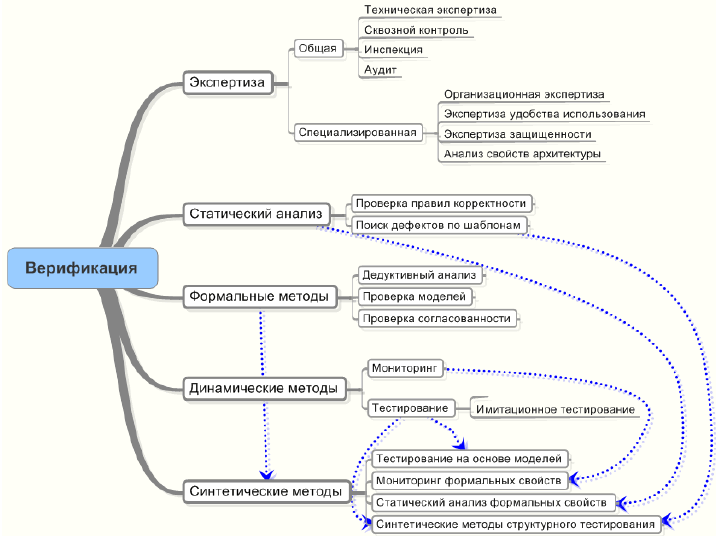
\includegraphics[width=\textwidth]{verification_classification.png}
    \end{center}
    \caption{Схема используемой классификации методов верификации}
    \label{fig:verification_classification}
\end{figure}

\newpage

\textbf{Экспертиза} позволяет находить ошибки, используя различные артефакты
жизненного цикла системы, в отличие от формальных и динамических методов, и
позволяет находить большое множество разновидностей ошибок. К ее недостаткам
можно отнести невозможность автоматизации.

\textbf{Статический анализ} - это процесс выявления ошибок и недочетов в
исходном коде программ. От остальных методов верификации его отделяет то, что
статический анализ использует только исходные тексты программы, что позволяет
обнаруживать ошибки на стадии написания кода. Таким образом, при анализе
отсутствует спецификация программы - описание того, что она делает. Это
уменьшает множество обнаруживаемых ошибок, но позволяет полностью
автоматизировать процесс анализа.

\textbf{Формальные методы} позволяют создавать формальные функциональные
спецификации и модели архитектуры систем, а также осуществлять их преобразование
в программы с последующей верификацией~\cite{formal_methods}. Корректность
полученных результатов гарантируется математическим аппаратом. К таким методам
относятся, например, дедуктивная верификация, проверка моделей и абстрактная
интерпретация.

Эти методы можно применить только к тем свойствам, которые можно выразить в
рамках некоторой математической модели. Построение этой модели не
автоматизируется, а провести анализ таких моделей может лишь специалист. Однако
сама проверка свойств может быть автоматизирована и позволяет находить даже
самые сложные ошибки.

\textbf{Динамические методы} используются для анализа и оценки свойств
программной системы по результатам ее реальной работы. Одними из таких методов
являются тестирование и анализ трасс исполнения.

Для применения данных методов необходимо иметь работающую систему (или ее
прототип), поэтому их нельзя использовать на ранних стадиях разработки. Также
данные методы позволяют найти только те ошибки в ПО, которые проявляются в его
работе.

\textbf{Синтетические методы} объединяют в себе элементы некоторых способов
повышения качества, описанных выше. Например, существуют динамические методы,
использующие элементы формальных - тестирование на основе моделей (model driven
testing)~\cite{Vieira2006} и мониторинг формальных свойств (runtime
verification)~\cite{runtime_verification}. Цель таких методов - объединить
преимущества уже используемых подходов.

%%%%%%%%%%%%%%%%%%%%%%%%%%%%%%%%%%%%%%%%%%%%%%%%%%%%%%%%%%%%%%%%%%%%%%%%%%%%%%%%
\section{Модели программных систем}
\label{sec:system_models}
%%%%%%%%%%%%%%%%%%%%%%%%%%%%%%%%%%%%%%%%%%%%%%%%%%%%%%%%%%%%%%%%%%%%%%%%%%%%%%%%

Одной из важнейших составляющих анализа программных систем является построение
модели. Без нее анализатор будет вынужден непосредственно оперировать с исходным
кодом, что влечет за собой усложнение процедур анализа и самого анализатора в
целом.

В зависимости от способа построения и назначения модели, они могу различаться по
структуре и сложности и обладать различными свойствами. Существуют следующие
виды моделей~\cite{itsykson}:

\begin{itemize}
    \item Структурные модели
    \item Поведенческие модели
    \item Гибридные модели
\end{itemize}

Структурные модели во основном используют информацию о синтаксической структуре
анализируемой программы, в то время как поведенческие - информацию о
динамической семантике. Гибридные модели используют оба этих подхода.

\subsubsection{Структурные модели}
\begin{enumerate}
    \item Синтаксическое дерево

    Синтаксическое дерево является результатом разбора программы в
    соответствии с формальной грамматикой языка программирования. Вершины
    этого дерева соответствуют нетерминальным символам грамматики, а листья
    - терминальным.

    \item Абстрактное синтаксическое дерево

    Данная модель получается из обычного синтаксического дерева путем
    удаления нетерминальных вершин с одним потомком и замены части
    терминальных вершин их семантическими атрибутами.
\end{enumerate}

\subsubsection{Поведенческие модели}

\nomenclature{AST}{Abstrac Syntax Tree, абстрактное синтаксическое дерево}
\nomenclature{CFG}{Control Flow Graph, граф потока управления}
\nomenclature{DDG}{Data Dependency Graph, граф зависимостей по данным}
\nomenclature{SSA}{Static Single Assignment, модель программы: однократное
статическое присваивание}

\begin{enumerate}
    \item Граф потока управления

    Граф потока управления представляет потоки управления программы в виде
    ориентированного графа. Вершинами графа являются операторы программы, а дуги
    отображают возможный ход исполнения программы и связывают между собой
    операторы, выполняемые друг за другом.

    \item Граф зависимостей по данным

    Граф зависимостей по данным отображает связь между конструкциями программы,
    зависимыми по используемым данным. Дуги графа соединяют узлы, формирующие
    данные, и узлы, использующие эти данные.

    \item Граф программных зависимостей

    Данная модель объединяет в себе особенности графа потока управления и графа
    зависимости по данным. В графе программных зависимостей присутствуют дуги
    двух типов: информационные дуги отображают зависимости по данным, а
    дуги управления соединяют последовательно выполняемые конструкции.

    \item Представление в виде SSA

    Однократное статическое присваивание (static single assignment) -
    промежуточное представление программы, которое обладает следующими
    свойствами:
        \begin{itemize}
            \item Всем переменным значение может присваиваться только один раз.
            \item Вводится специальный оператор $\phi$-функция, который
            объединяет разные версии локальных переменных.
            \item Все операторы программы представляются в трехоперандной форме.
        \end{itemize}
\end{enumerate}

\subsubsection{Гибридные модели}
\begin{enumerate}
    \item Абстрактный семантический граф

    Данная модель является расширением абстрактного синтаксического дерева путем
    добавления дуг, отражающих некоторые семантически свойства программы,
    например, такие дуги могут связывать определение и использование переменной
    или определение функции и ее вызов.
\end{enumerate}

\todo{Рассказать про метамодели и их положение в иерархии моделирования}

%%%%%%%%%%%%%%%%%%%%%%%%%%%%%%%%%%%%%%%%%%%%%%%%%%%%%%%%%%%%%%%%%%%%%%%%%%%%%%%%
\section{Анализ существующих решений}
\label{sec:analysis}
%%%%%%%%%%%%%%%%%%%%%%%%%%%%%%%%%%%%%%%%%%%%%%%%%%%%%%%%%%%%%%%%%%%%%%%%%%%%%%%%

Обощенное решение задач анализа и верификации основывается на использовании
метамоделей~\cite{metamodeling} - описаний модели системы, имеющих различные
уровни детализации в зависимости от преследуемых целей.

На данный момент существует лишь небольшое количество инструментов, использующих
метамоделирование. Рассмотрим их подробнее.

%%%%%%%%%%%%%%%%%%%%%%%%%%%%%%%%%%%%%%%%%%%%%%%%%%%%%%%%%%%%%%%%%%%%%%%%%%%%%%%%
\subsubsection{Moose}
%%%%%%%%%%%%%%%%%%%%%%%%%%%%%%%%%%%%%%%%%%%%%%%%%%%%%%%%%%%%%%%%%%%%%%%%%%%%%%%%
\nomenclature{Moose}{Платформа для анализа программ}

Moose является платформой для анализа программ и поддерживает большое количество
различных видов анализа~\cite{moose}:

\begin{enumerate}
    \item Построение и визуализация метрик.
    \item Обнаружение клонов.
    \item Построение графа зависимостей между пакетами.
    \item Вывод словаря, используемого в проекте.
    \item Поддержка браузеров исходного кода.
\end{enumerate}

\nomenclature{FAMIX}{Семейство метамоделей, используемых средством Moose}
\nomenclature{XML}{eXtensible Markup Language, расширяемый язык разметки}
\nomenclature{MSE}{язык разметки, используемый средством Moose}

Moose использует целое семейство метамоделей под названием FAMIX. Данное
семейство обладает довольно сложной структурой, упрощенный вид которой приведен
на рис~\ref{fig:famix_hierarchy}

\newpage
\begin{figure}[h!]
     \begin{center}
         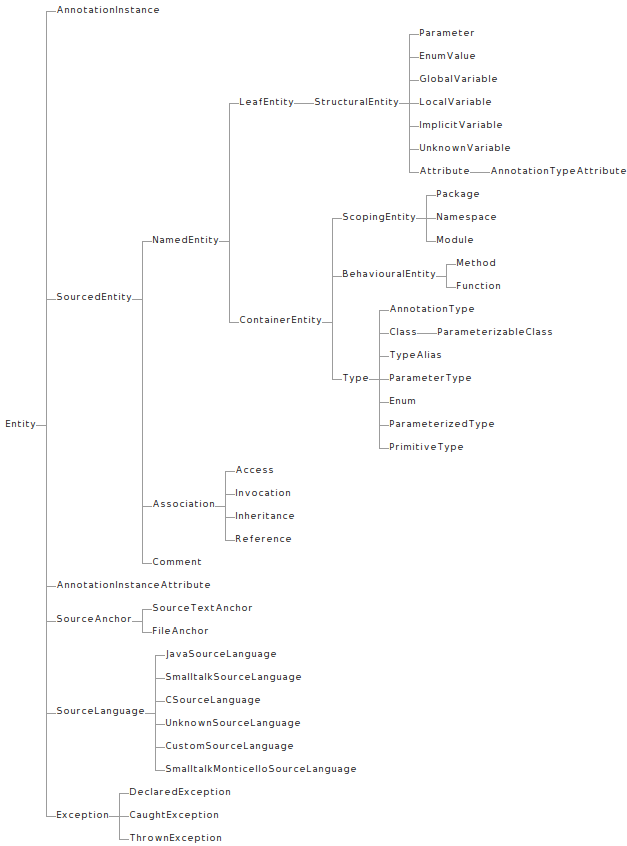
\includegraphics[width=0.9\textwidth]{famix_hierarchy.png}
     \end{center}
     \caption{Структура метамоделей семейства FAMIX}
     \label{fig:famix_hierarchy}
\end{figure}
\newpage

Анализ программы происходит следующим образом:

\begin{enumerate}
    \item Импортирование входных данных. Импортирование может происходить как
    при помощи встроенных средств (Moose поддерживает Smalltalk, XML и MSE),
    так и при помощи сторонних средств.
    \item После импортирования данные приводятся к одной из метамоделей
    семейства FAMIX.
    \item Применение заданных алгоритмов анализа.
\end{enumerate}

Архитектура средства приведена на рис~\ref{fig:moose_architecture}

\begin{figure}[h]
    \begin{center}
        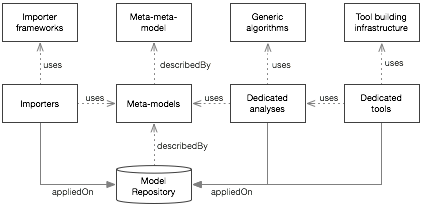
\includegraphics[width=\textwidth]{moose_architecture.png}
    \end{center}
    \caption{Архитектура фреймворка Moose}
    \label{fig:moose_architecture}
\end{figure}

К недостаткам данной среды, можно отнести то, что Moose нацелен в первую очередь
на задачи реинжиниринга и обладает слишком избыточной и громоздкой метамоделью
для разработки на ее основе алгоритмов статического анализа и верификации.

%%%%%%%%%%%%%%%%%%%%%%%%%%%%%%%%%%%%%%%%%%%%%%%%%%%%%%%%%%%%%%%%%%%%%%%%%%%%%%%%
\subsubsection{SMIILE}
%%%%%%%%%%%%%%%%%%%%%%%%%%%%%%%%%%%%%%%%%%%%%%%%%%%%%%%%%%%%%%%%%%%%%%%%%%%%%%%%

\nomenclature{SMIILE}{Software Metrics Independent of Input LanguagE,
средство для анализа программ}

\nomenclature{eCST}{enriched Concrete Syntax Tree, модель программы,
используемая средством SMIILE}

SMIILE - среда, предназначенная для вычисления метрик анализируемой
системы~\cite{smile}.

В качестве метамодели SMIILE использует представление в виде eCST (enriched
Concrete Syntax Tree), которое представляет собой дерево разбора программы с
добавлением универсальных узлов, что позволяет сделать дерево разбора
независимым от входного языка программирования.

На рис~\ref{fig:smile_arch} изображена архитектура данного средства:

\begin{figure}[h!]
    \begin{center}
        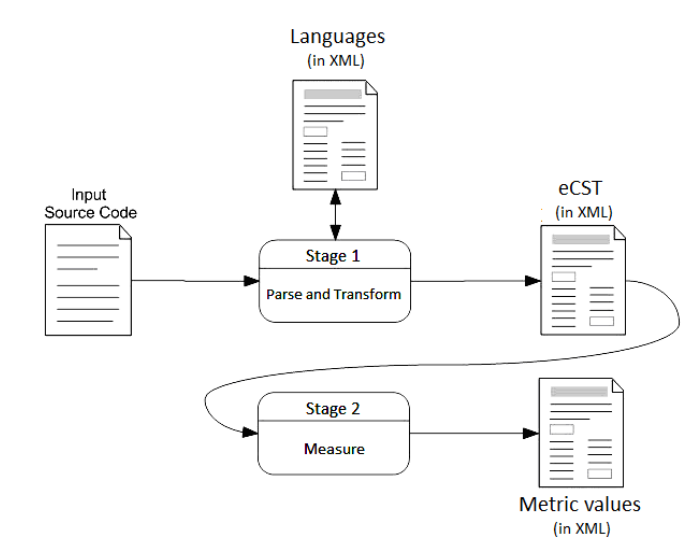
\includegraphics[width=0.8\textwidth]{smile_arch.png}
    \end{center}
    \caption{Архитектура SMIILE}
    \label{fig:smile_arch}
\end{figure}

Анализ программы происходит в две фазы:

\begin{enumerate}
    \item Фаза 1
    \begin{itemize}
        \item Определение языка программирования, на котором написана
        анализируемая программа.
        \item Вызов парсера этого языка для построения CST и преобразование в
        eCST.
        \item Вывод результата в формате XML.
    \end{itemize}

    \item Фаза 2
    \begin{itemize}
        \item Считывание eCST из файла.
        \item Подсчет метрик.
        \item Сохранение результата в формате XML.
    \end{itemize}
\end{enumerate}

Средство SMILE на данный момент не разрабатывается и, помимо подсчета метрик, не
предоставляет никаких других возможностей.

%%%%%%%%%%%%%%%%%%%%%%%%%%%%%%%%%%%%%%%%%%%%%%%%%%%%%%%%%%%%%%%%%%%%%%%%%%%%%%%%
\subsubsection{LLVM}
%%%%%%%%%%%%%%%%%%%%%%%%%%%%%%%%%%%%%%%%%%%%%%%%%%%%%%%%%%%%%%%%%%%%%%%%%%%%%%%%

\nomenclature{LLVM}{Low Level Virtual Machine, фреймворк для создания
компиляторов}

LLVM - фреймворк для анализа и трансформации программ, путем предоставления
информации для трансформаций компилятору во время компиляции, линковки и
исполнения~\cite{llvm}.

LLVM использует промежуточное представление, в основе которого лежит
представление в виде SSA. Промежуточное представление является набором
RISC-подобных команд и содержит дополнительную информацию более высокого уровня,
например информацию о типах и графе потока управления.

Данный фреймворк обладает следующими особенностями:

\begin{enumerate}
    \item Сохранение информации о программе даже во время исполнения и между
    запусками.
    \item Предоставление информации пользователю для профилирования и
    оптимизации.
    \item Промежуточное представление не зависит от языка программирования.
    \item Возможность оптимизации всей системы в целом (после этапа линковки).
\end{enumerate}

Архитектура LLVM приведена на рис~\ref{fig:llvm_arch}:

\newpage

\begin{figure}[h!]
    \begin{center}
        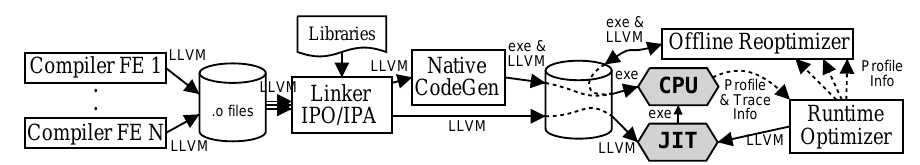
\includegraphics[width=\textwidth]{llvm_arch.png}
    \end{center}
    \caption{Архитектура LLVM}
    \label{fig:llvm_arch}
\end{figure}

Front-end компиляторы транслируют исходную программу в промежуточное
представление LLVM, которое затем компонуется LLVM-линкером. На этой стадии
может проводиться межпроцедурный анализ. Получившийся код затем транслируется
в машинный код для целевой платформы.

Однако, промежуточное представление, используемое в LLVM, обладает
недостаточной полнотой описания, необходимой для подсчета метрик и визуализации
свойств программной системы.

%%%%%%%%%%%%%%%%%%%%%%%%%%%%%%%%%%%%%%%%%%%%%%%%%%%%%%%%%%%%%%%%%%%%%%%%%%%%%%%%
\subsubsection{ULF-Ware}
%%%%%%%%%%%%%%%%%%%%%%%%%%%%%%%%%%%%%%%%%%%%%%%%%%%%%%%%%%%%%%%%%%%%%%%%%%%%%%%%

\nomenclature{ULF-Ware}{Unified Language Family softWare, фреймворк для
генерации кода из программных моделей}

\nomenclature{SDL}{Specification and Description Language, язык для описания
моделей программных систем}

ULF-Ware является средством для генерации кода из модели, созданной при помощи
языка SDL (Specification and Description Language)~\cite{metamodeling}. Данное
средство использует метамодель под названием CeeJay, которая предназначена для
описания систем на языках Java и C++.

Архитектура ULF-Ware приведена на рис~\ref{fig:ulf_ware_arch}:

\newpage

\begin{figure}[h!]
    \begin{center}
        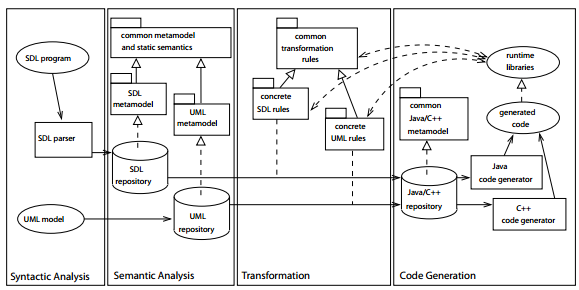
\includegraphics[width=\textwidth]{ulf_ware_arch.png}
    \end{center}
    \caption{Архитектура ULF-Ware}
    \label{fig:ulf_ware_arch}
\end{figure}

Генерация кода происходит следующим образом: компилятор SDL создает модель
программы, полученную из SDL-описания, соответствующую метамодели SDL. После
этого происходит трансформация исходной модели в экземпляр метамодели CeeJay,
который обладает всей необходимой информацией для генерации кода на языке Java
или C++.

Ограничением данного средства и метамодели CeeJay является тот факт, что, в силу
специфики задачи, данная метамодель может применяться только для языков Java и
C++.
